\documentclass{beamer}

%%%%%%%%%%%%%Solarized Theme%%%%%%%%%%%%%%%
\usecolortheme[dark,accent=cyan]{solarized}
\beamertemplatenavigationsymbolsempty

%%%%%Packages%%%%%
\usepackage{varwidth}
\usepackage{hyperref}

\usepackage{tikz}
\usepackage{standalone}
\usetikzlibrary{positioning,calc}
\usetikzlibrary{automata}
\usetikzlibrary{fit}                    % fitting shapes to coordinates
\usetikzlibrary{backgrounds}    % drawing the background after the foreground

\tikzstyle{background}=[orange, rectangle, draw, inner sep=0.2mm,
           rounded corners=1mm, ultra thick]
\usepackage{minted}

\definecolor{DarkGray}{gray}{0.1}
\usemintedstyle{native}

\title{Arcas: Using Python to access open research literature}
\author{@NikoletaGlyn}
\date{ }
\institute[]
{
\begin{center}
    
\includegraphics[width=.20\textwidth]{static/euroscipy-logo.png}
    \hspace{0.5cm}
\includegraphics[width=.20\textwidth]{static/arcas-logo.jpg}
\end{center}
}

\begin{document}

\frame{\titlepage}

\begin{frame}
    \begin{center}
    
\includegraphics[width=0.24\textwidth]{static/cardiff_uni_logo.jpg}\hspace{10pt}
    
\includegraphics[width=0.24\textwidth]{static/axelrod-logo.png}\vspace{10pt}

    \hspace{3pt} 
\includegraphics[width=0.24\textwidth]{static/ssi-logo.png}
    \end{center}
\end{frame}

\begin{frame}
\begin{center}
\textcolor{orange}{
\huge{The illustrated guide to a Ph.D.} \\
\vspace{10mm}
\large{Matt Might} \\}
\vspace{10mm}
\small{http://matt.might.net/articles/phd-school-in-pictures/}
\end{center}
\end{frame}

\begin{frame}
    \begin{center}
    \tikzstyle{arrow} = [thick,->,>=stealth]

\begin{center}
\begin{tikzpicture}

\draw (0, 0) circle (3cm);
\draw[blue!70,fill=blue!70] (0, 0) circle (0.5cm);
\draw[line width=1mm, yellow!70](0, 0) circle (0.8);
\draw [arrow, line width=0.5mm, red!70] (0.5, 0.7) -- (0.7, 1);
\draw [arrow, line width=0.5mm, red!40] (0.5, 0.7) -- (0.7, 1);
\draw [arrow, line width=0.5mm, red!60] (0.7, 1) -- (.95, 1.4);

\draw [arrow, line width=0.5mm, red!80] (0.95, 1.4) -- (1.67, 2.5);

\end{tikzpicture}
\end{center}
    \end{center}
\end{frame}

\begin{frame}
    \centering
    \includestandalone[width=0.9\textwidth]{static/process}
\end{frame}

\begin{frame}
\begin{center}
\textcolor{orange}{
    \Huge{Sustainable Software}}
\end{center}
\end{frame}

\begin{frame}
\begin{center}
    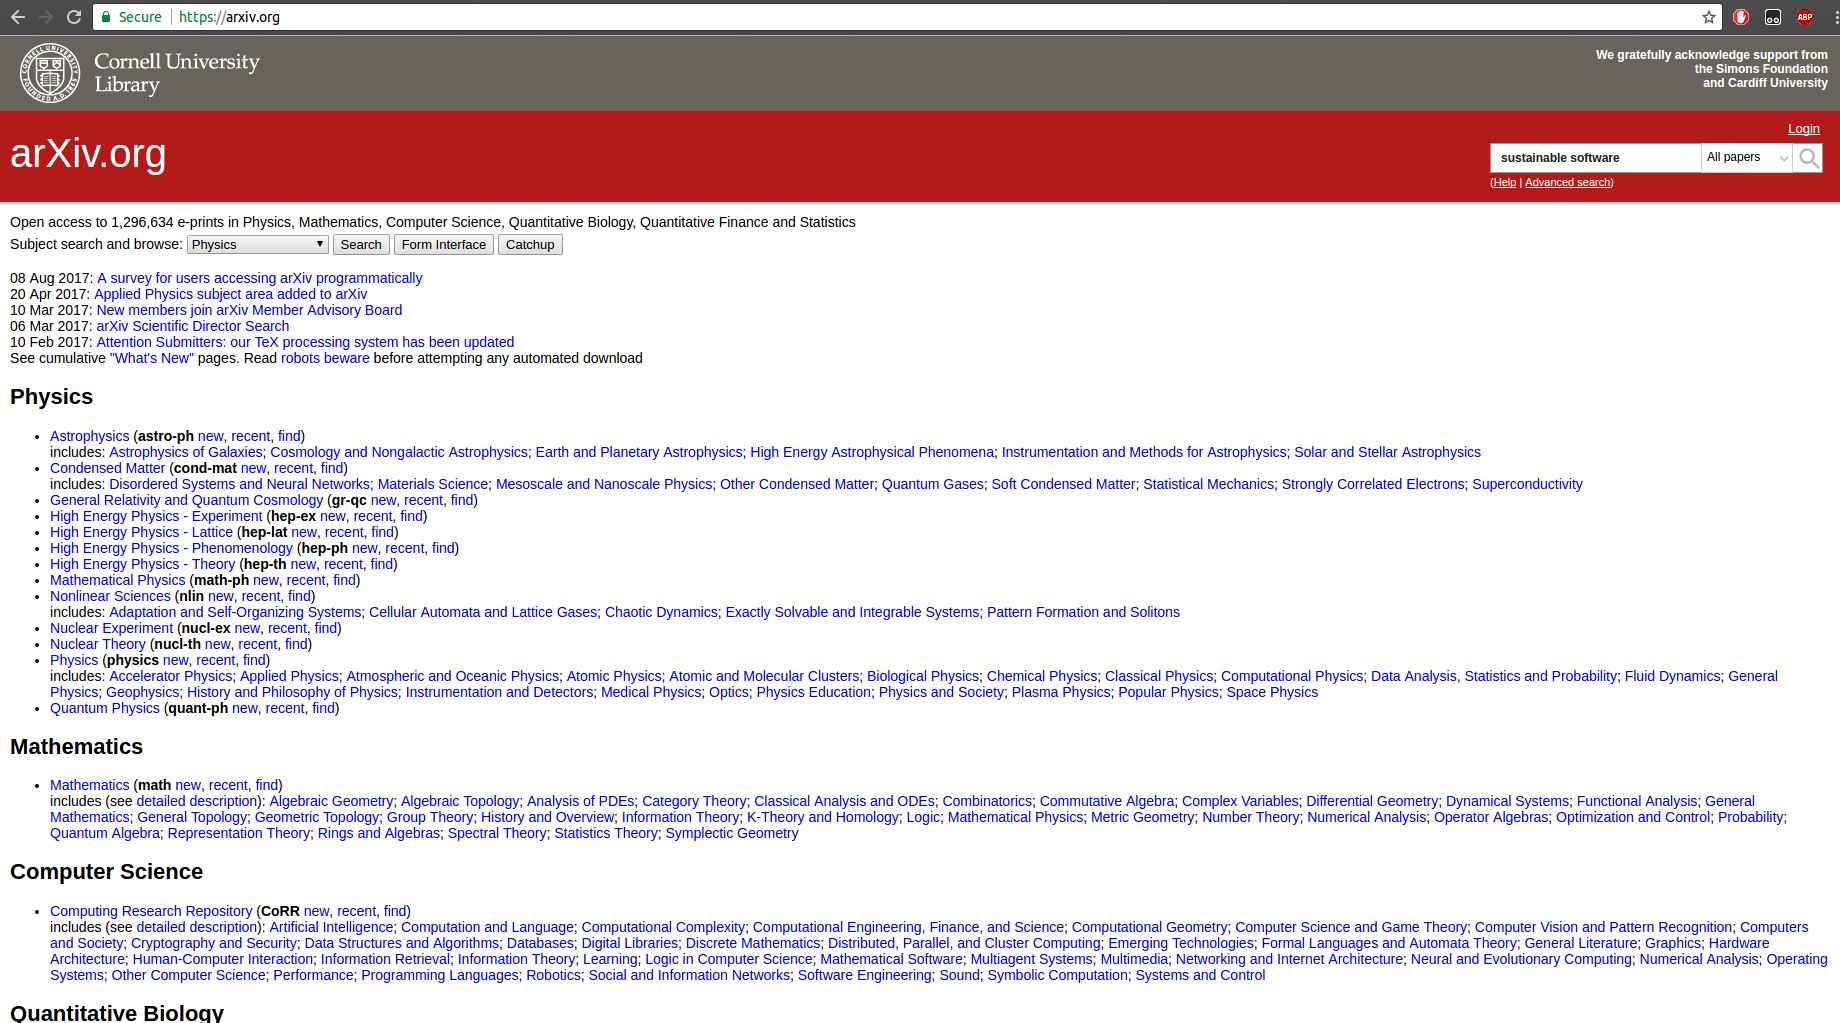
\includegraphics[width=\textwidth, height=0.5\textwidth]{static/arxiv_search.png}
\end{center}
\end{frame}

\begin{frame}
\begin{center}
    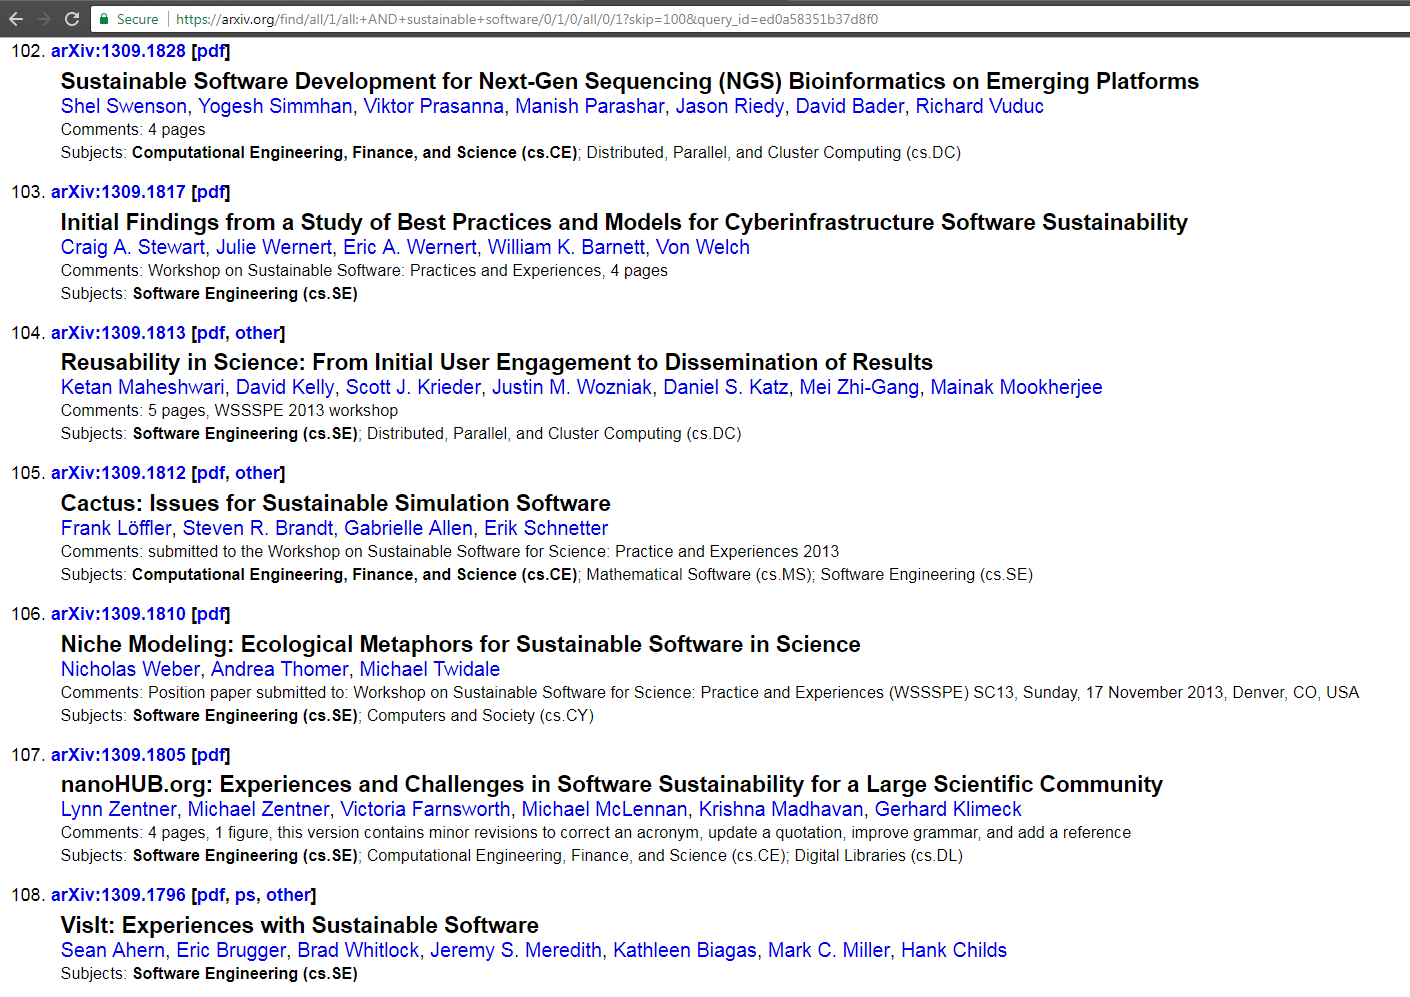
\includegraphics[width=\textwidth]{static/arxiv_result.png}
\end{center}
\end{frame}

\begin{frame}
\begin{center}
\color{orange}\Large{$0.5 \textrm{min} + \textrm{100} \times 1.5 \textrm{min} + 10 \times 0.5
\textrm{min}= 155.5 \textrm{min} \Rightarrow 2 \textrm{h} \textrm{ and } 35.5
\textrm{min}$}
\end{center}
\end{frame}

\begin{frame}
\begin{center}
\textcolor{orange}{
\Huge{API}}
\end{center}
\end{frame}

\begin{frame}[fragile]
    \centering
    \textcolor{orange}{\textbf{QUERY}} \\
    \vspace{3mm}
    \small{\url{http://export.arxiv.org/api/query?search_query=ti:Sustainable%20Software}} \\
\end{frame}

\begin{frame}
\begin{center}
    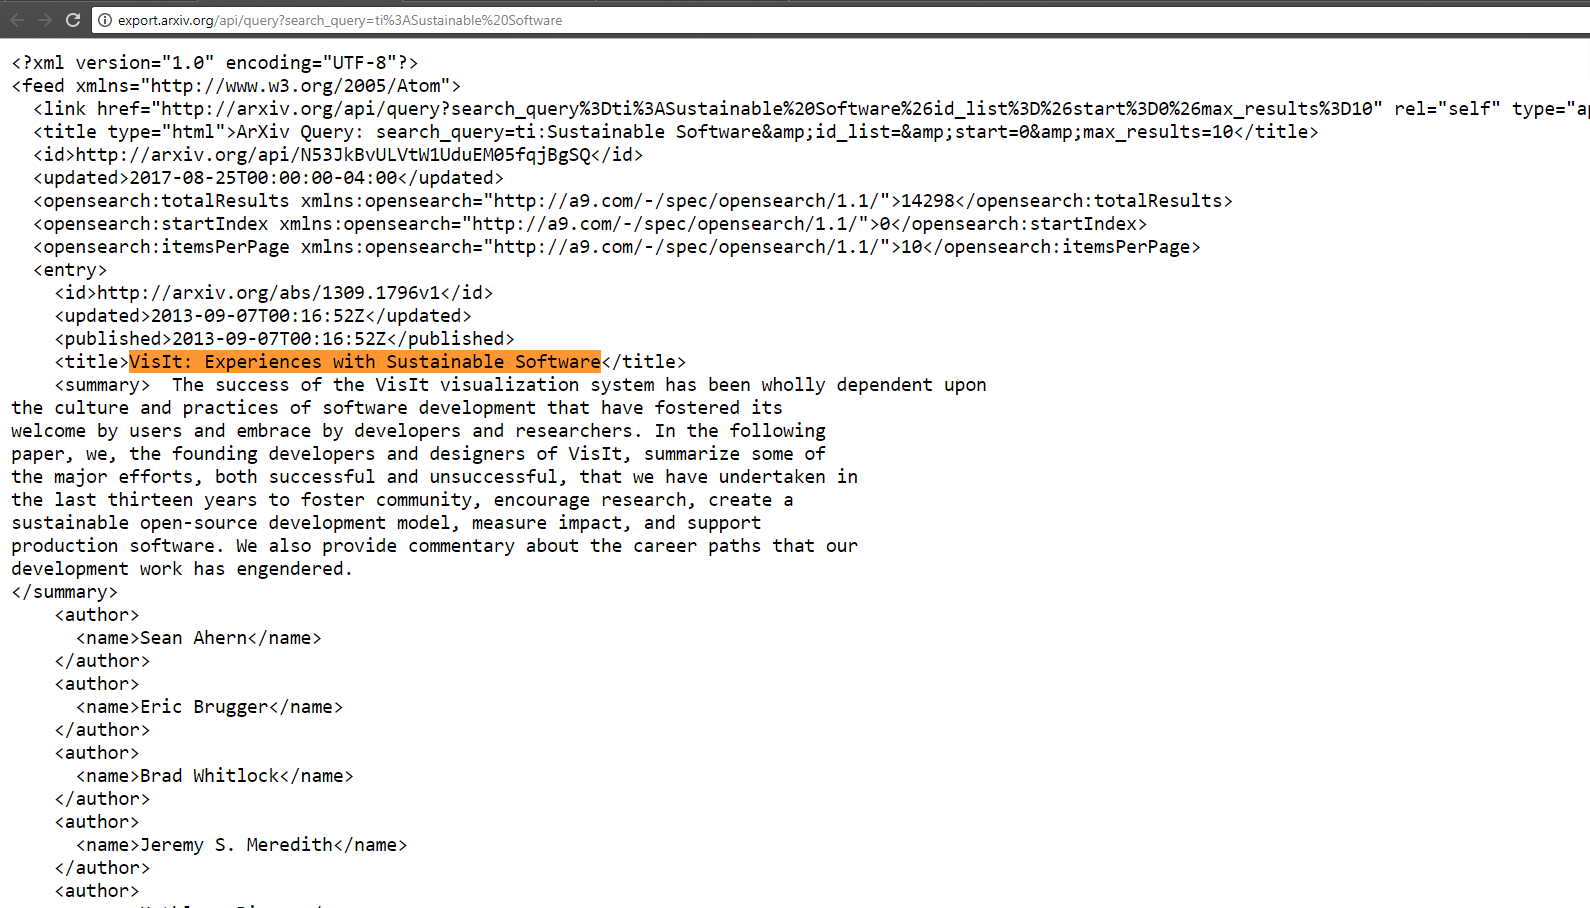
\includegraphics[width=\textwidth]{static/arxiv_api_result.png}
\end{center}
\end{frame}

\begin{frame}
\begin{center}
\color{orange}\Large{$15 \textrm{min} + 1 \textrm{min} + 50 \textrm{min} =
66 \textrm{min} \Rightarrow 1\textrm{h} \textrm{ and } 6 \text{min}$}
\end{center}
\end{frame}

\begin{frame}[fragile]
    \begin{center}
    \textcolor{orange}{\textbf{QUERY}} \\
    \vspace{3mm}
    \small{\url{http://export.arxiv.org/api/query?search_query=ti:Sustainable%20Software}} \\
    \pause
    \vspace{10mm}
    \small{\url{http://api.plos.org/search?q=title:Sustainable%20Software&rows=100}} \\
    \pause
    \vspace{10mm}
    \small{\url{http://www.nature.com/opensearch/request?queryType=cql&query=dc
    .title%20adj%20SustainableSoftware&maximumRecords=100}} \\
    \small{...}
    \end{center}
\end{frame}

\begin{frame}
    \begin{center}
    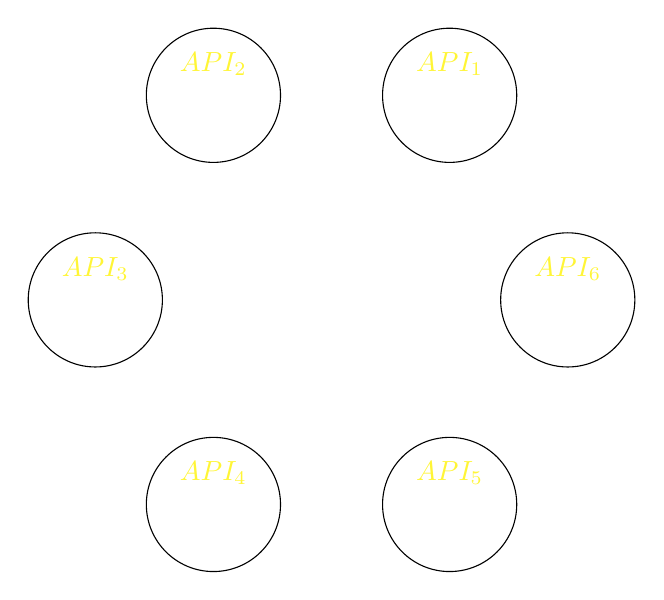
\begin{tikzpicture}

\foreach \phi in {1,...,6}{
    \node[state, align=center] (v_\phi) at (360/6 * \phi:3cm) {\color{yellow!79}$API_\phi$ \\\color{white!79}\tiny{Query}
    \\ \color{white!79}\tiny{XML}};
}
\end{tikzpicture}
    \end{center}
\end{frame}
\begin{frame}[fragile]
    \begin{center}
    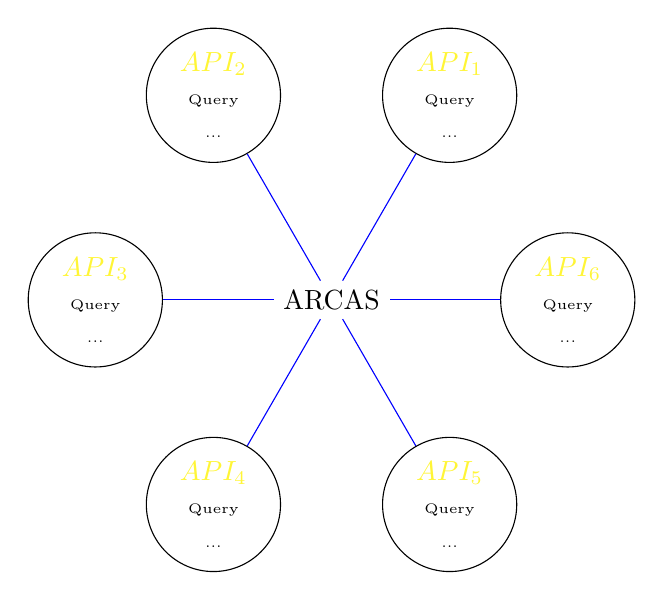
\begin{tikzpicture}

    \node (center) at (0,0) {ARCAS};
\foreach \phi in {1,...,6}{
    \node[state, align=center] (v_\phi) at (360/6 * \phi:3cm) {\color{yellow!79}$API_\phi$ \\ \tiny{Query} \\ \tiny{...}};
         \draw[blue] (v_\phi) -- (center);
}
\end{tikzpicture}
    \end{center}
\end{frame}

\begin{frame}[fragile]
    \begin{minted}
    [
    framesep=4mm,
    baselinestretch=1.2,
    bgcolor=DarkGray,
    fontsize=\footnotesize,
    ]
    {python}
$ pip install arcas

    \end{minted}
\end{frame}

\begin{frame}[fragile]

    \begin{minted}
    [
    framesep=4mm,
    baselinestretch=1.2,
    bgcolor=DarkGray,
    fontsize=\footnotesize,
    ]
    {python}
>>> import arcas

>>> api = arcas.Arxiv()
>>> parameters = api.parameters_fix(
...     title='sustainable software', records=1, start=1)
>>> url = api.create_url_search(parameters)
>>> request = api.make_request(url)
>>> root = api.get_root(request)
>>> raw_article = api.parse(root)

>>> article = api.to_dataframe(raw_article[0])
>>> api.export(article, "result.json")

    \end{minted}
\end{frame}

\begin{frame}[fragile]

    \begin{minted}
    [
    framesep=4mm,
    baselinestretch=1.2,
    bgcolor=DarkGray,
    fontsize=\footnotesize,
    ]
    {python}
{"key":{"0":"Ahern2013"},
 "unique_key":{"0":"698d27415f69258ef122f46b184a77e0"},
 "title":{"0":"VisIt: Experiences with Sustainable Software"},
 "author":{"0":"Sean Ahern","1":"Eric Brugger"},
 "abstract":{"0":"  The success of the VisIt visualization..."},
 "date":{"0":2013},
 "journal":{"0":"arXiv"},
 "provenance":{"0":"arXiv"}}
    \end{minted}
\end{frame}

\begin{frame}[fragile]
    \begin{minted}
    [
    framesep=4mm,
    baselinestretch=1.2,
    bgcolor=DarkGray,
    fontsize=\scriptsize,
    ]
    {python}
>>> for p in [arcas.Arxiv, arcas.Nature, arcas.Ieee, arcas.Plos]:
...    api = p()
...    parameters = api.parameters_fix(
...         title='sustainable software', records=1, start=1)
...    url = api.create_url_search(parameters)
...    request = api.make_request(url)
...    root = api.get_root(request)
...    raw_article = api.parse(root)
...    try:
...        for art in raw_article:
...            article = api.to_dataframe(art)         
...        api.export(article, "result_from_{}.json".format(
...            api.__class__.__name__))    
...    except TypeError:
...        pass

    \end{minted}
\end{frame}

\begin{frame}
\begin{center}
\color{orange}\Large{$15 \textrm{min} + 5 \textrm{min} = 20 \textrm{min}$}
\end{center}
\end{frame}

\begin{frame}
\begin{center}
    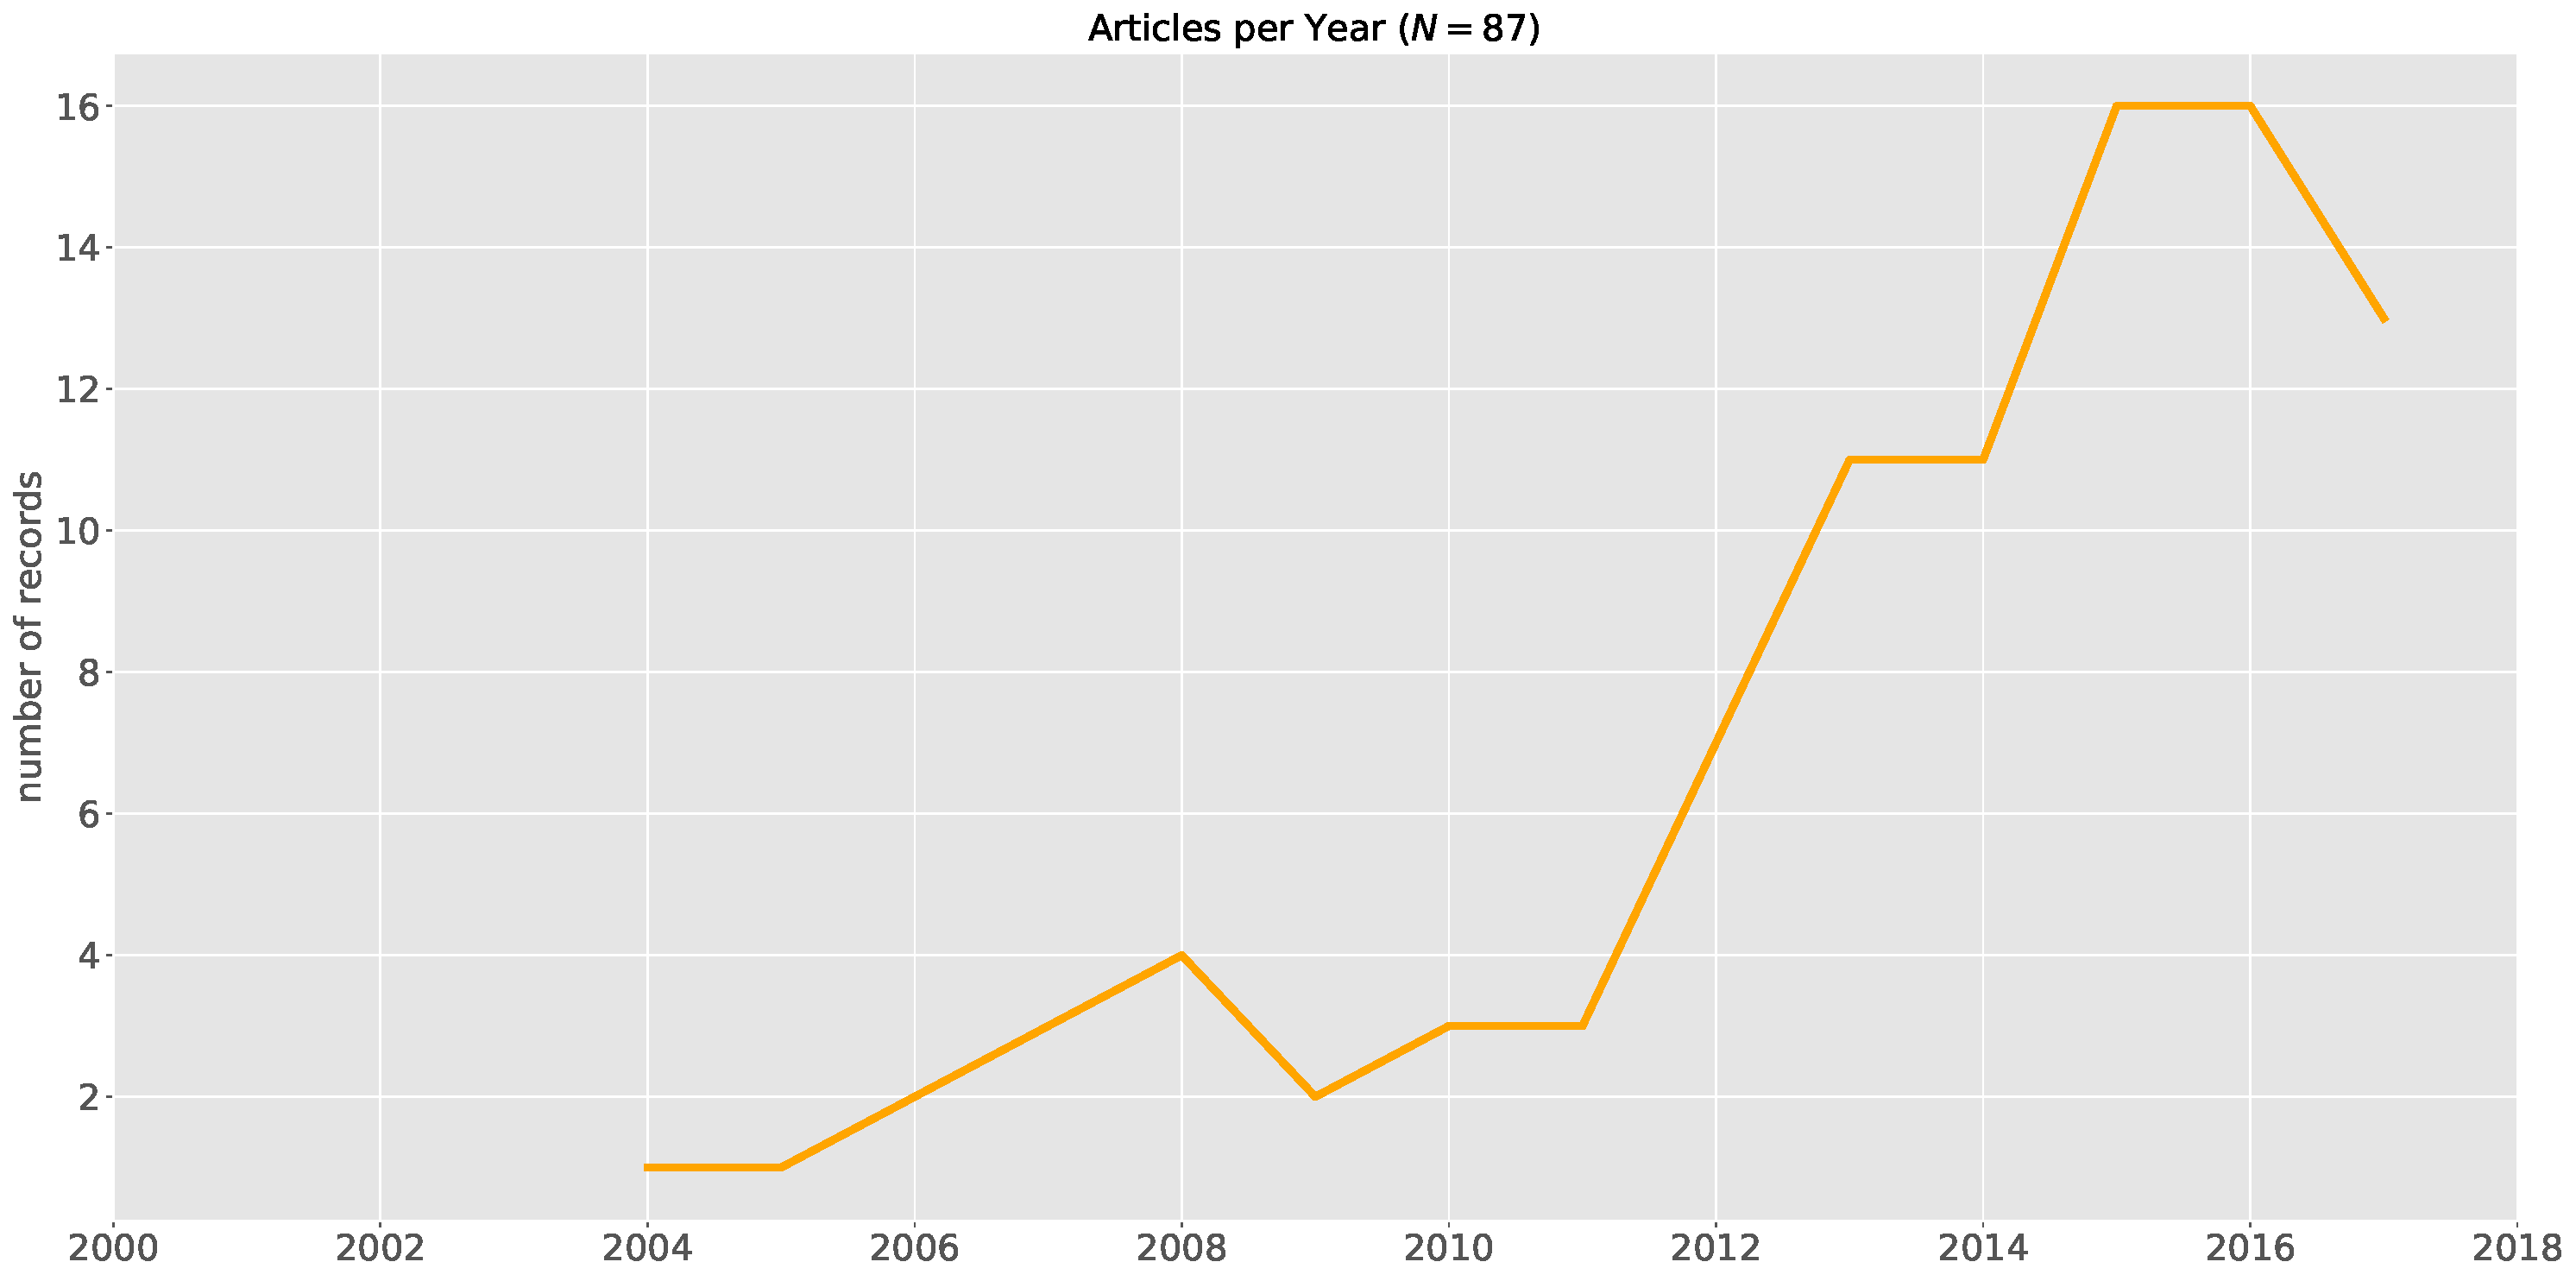
\includegraphics[width=\textwidth]{static/timeline.pdf}
\end{center}
\end{frame}

\begin{frame}
\begin{center}
    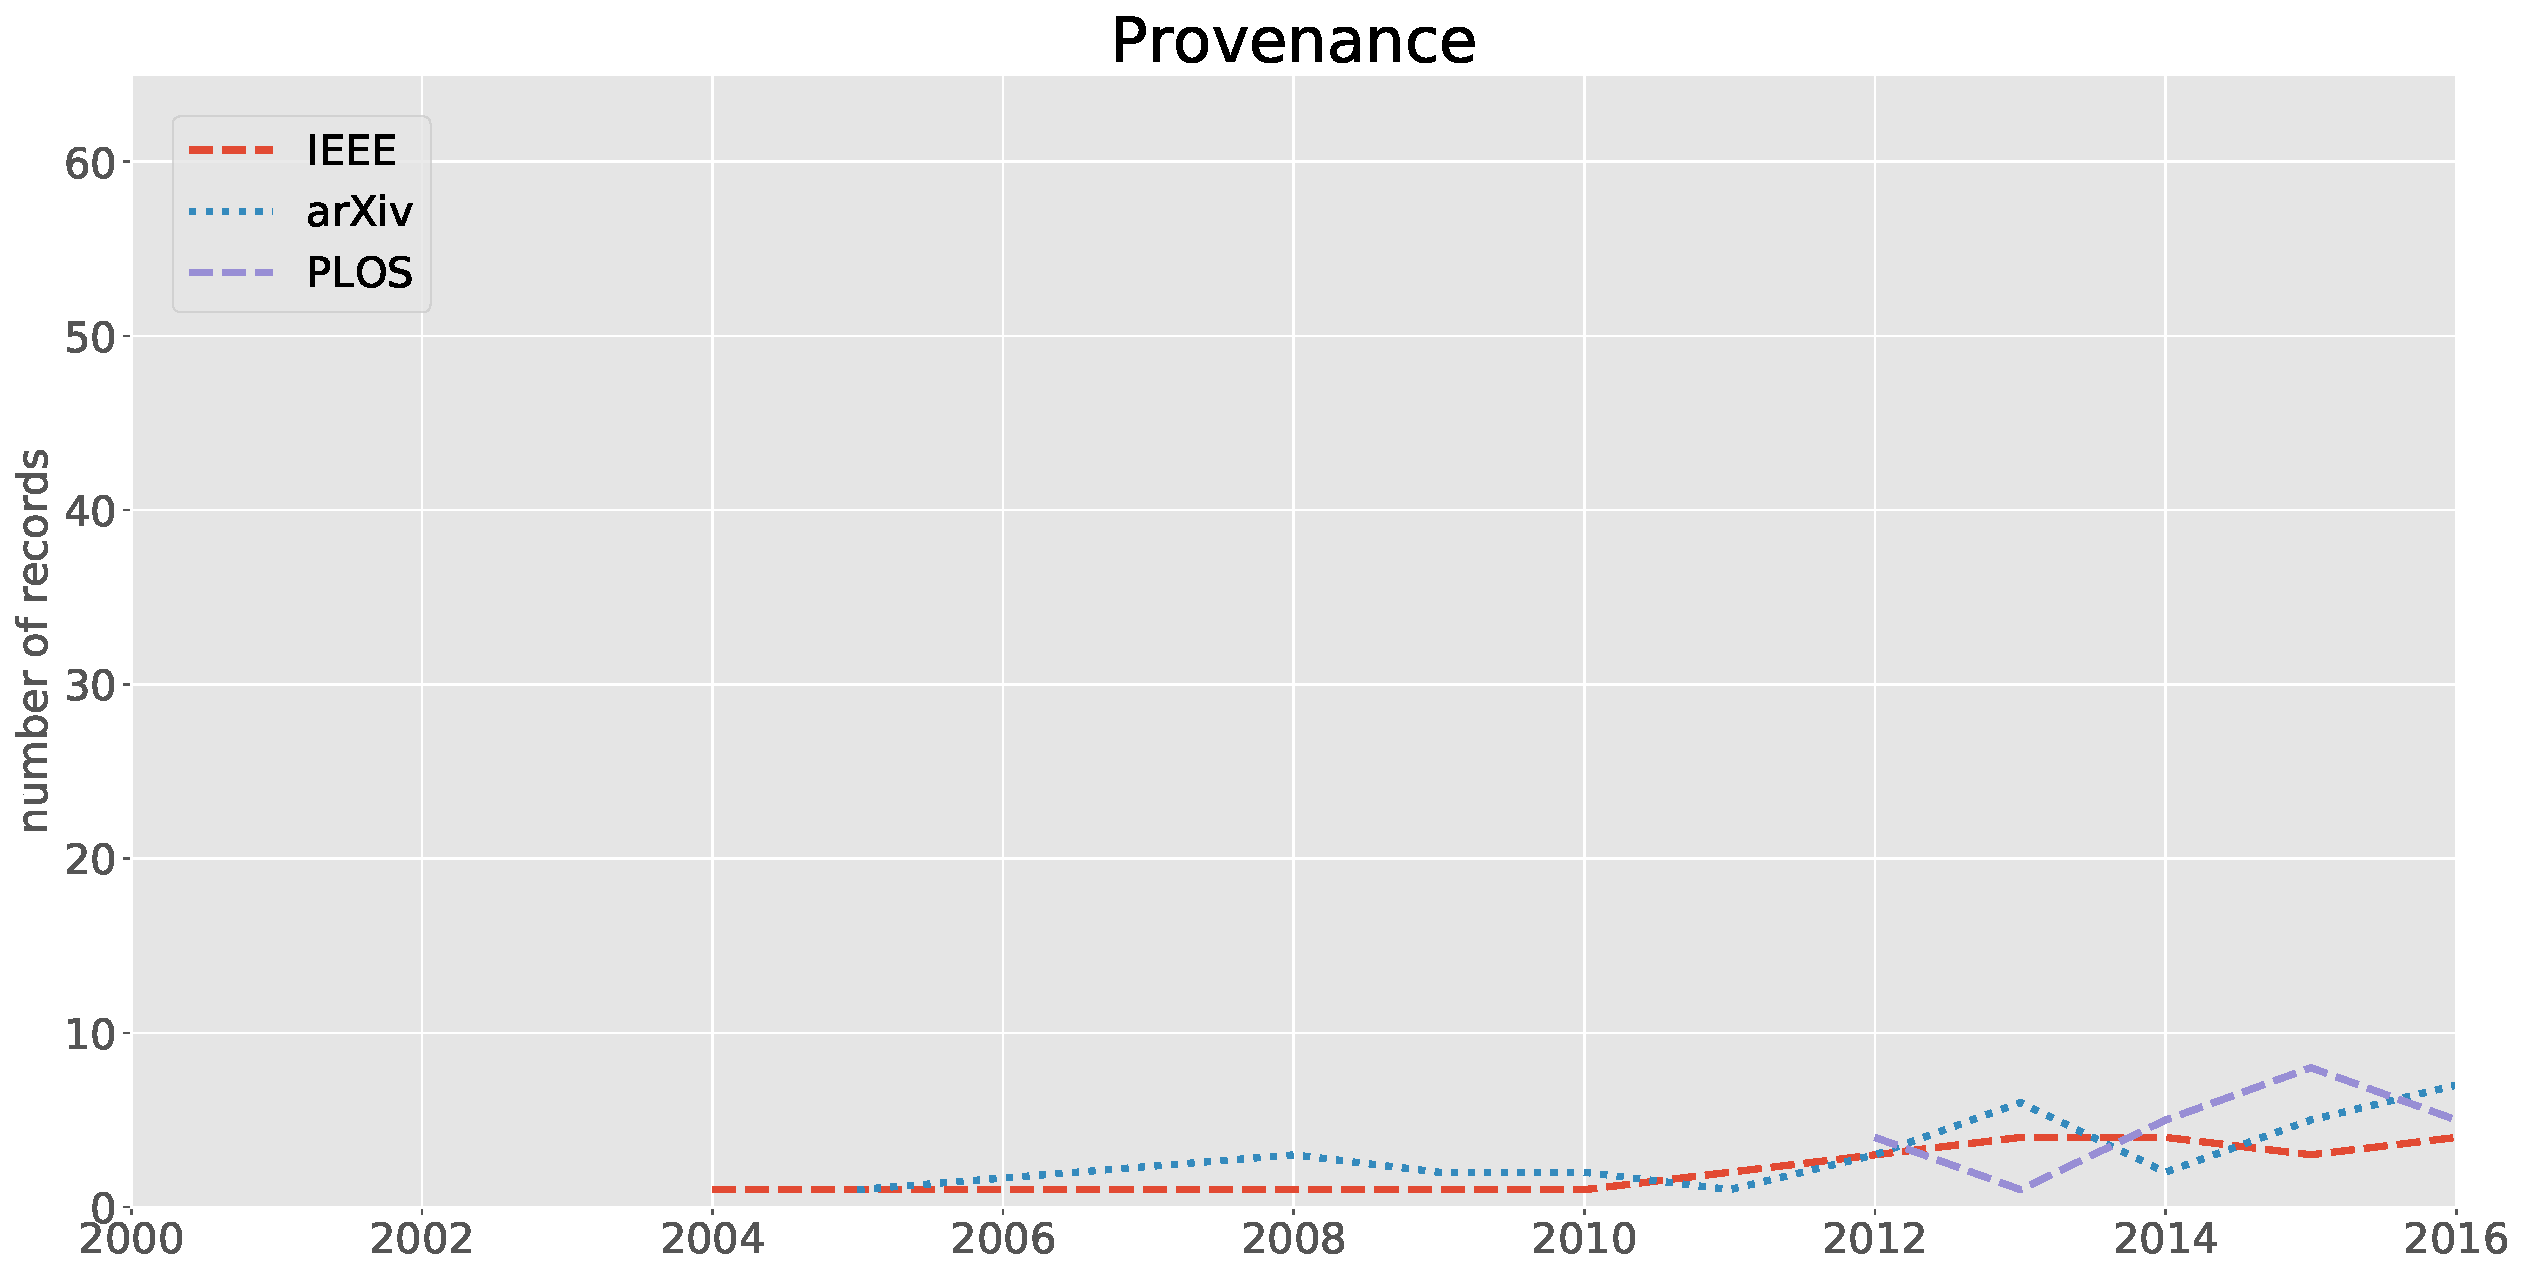
\includegraphics[width=\textwidth]{static/provenance.pdf}
\end{center}
\end{frame}

\begin{frame}
\begin{center}
    \includegraphics[width=0.8\textwidth]{static/network.pdf}
\end{center}
\end{frame}

\begin{frame}
\begin{center}
    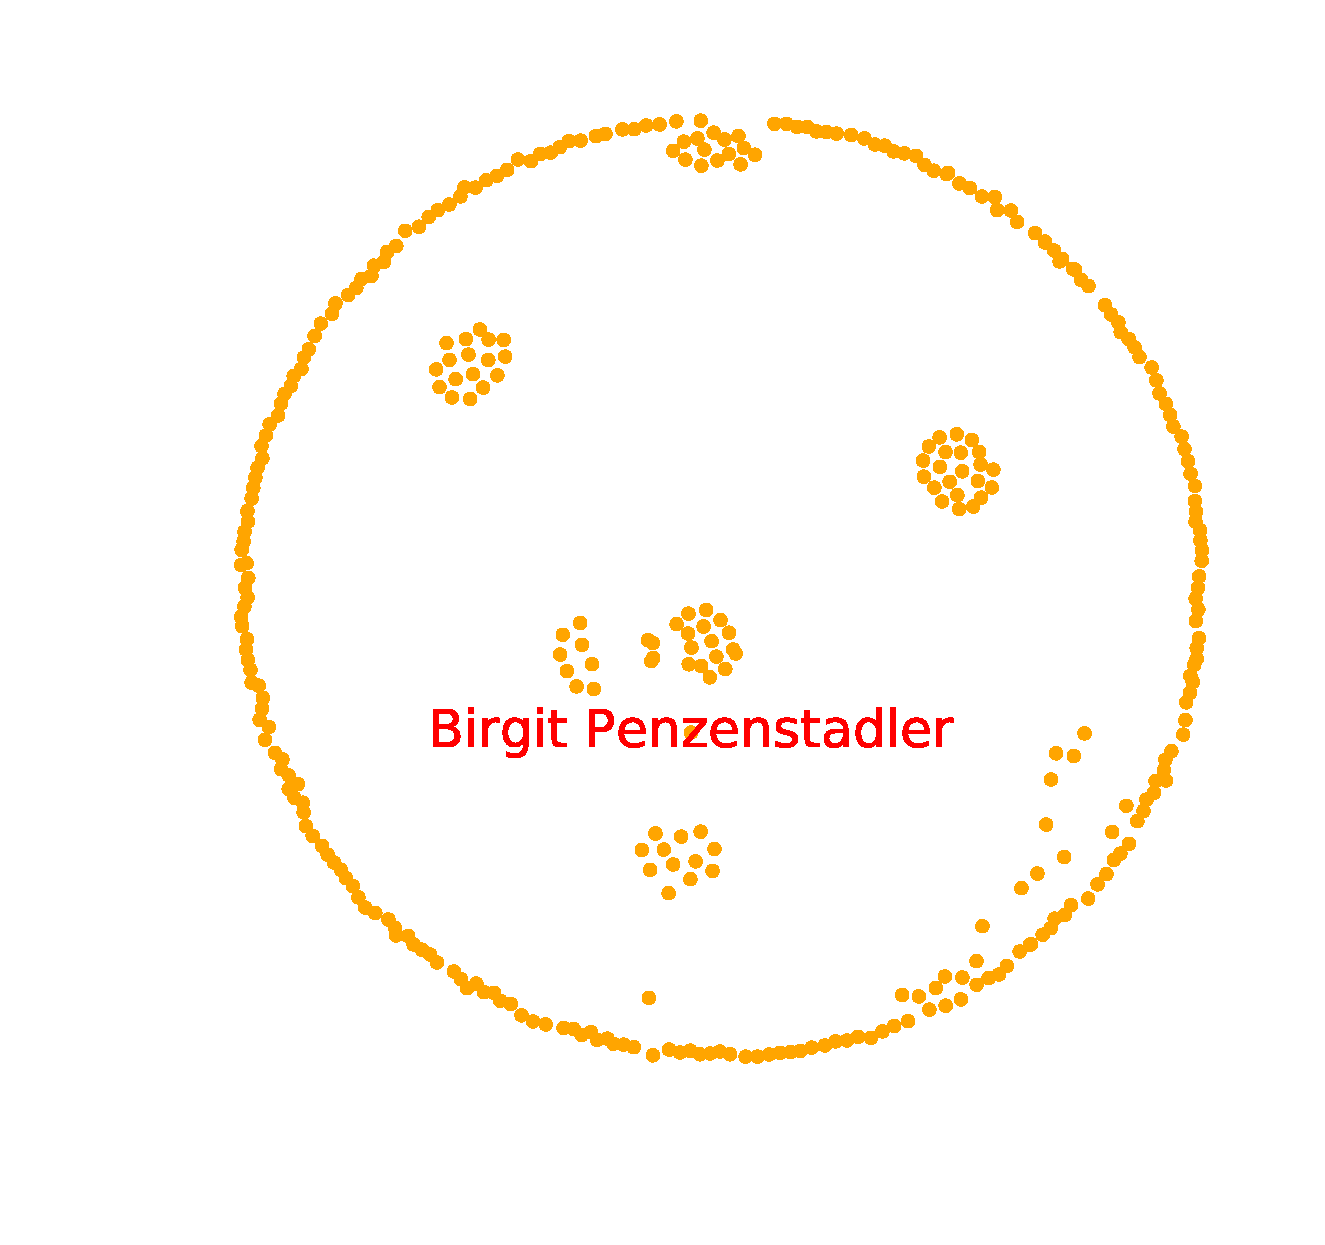
\includegraphics[width=0.8\textwidth]{static/network_2.pdf}
\end{center}
\end{frame}

\begin{frame}
\centering
\textcolor{brown}{\large{Arcas}}
\begin{center}
\begin{figure}
    \documentclass{standalone}

\usepackage{tikz}
\usepackage{standalone}
\usetikzlibrary{calc}
\usetikzlibrary{decorations.pathmorphing}
\usetikzlibrary{fit}                    % fitting shapes to coordinates
\usetikzlibrary{backgrounds}    % drawing the background after the foreground

\tikzstyle{background}=[orange, rectangle, draw, inner sep=0.2mm,
           rounded corners=1mm, ultra thick]

\begin{document}
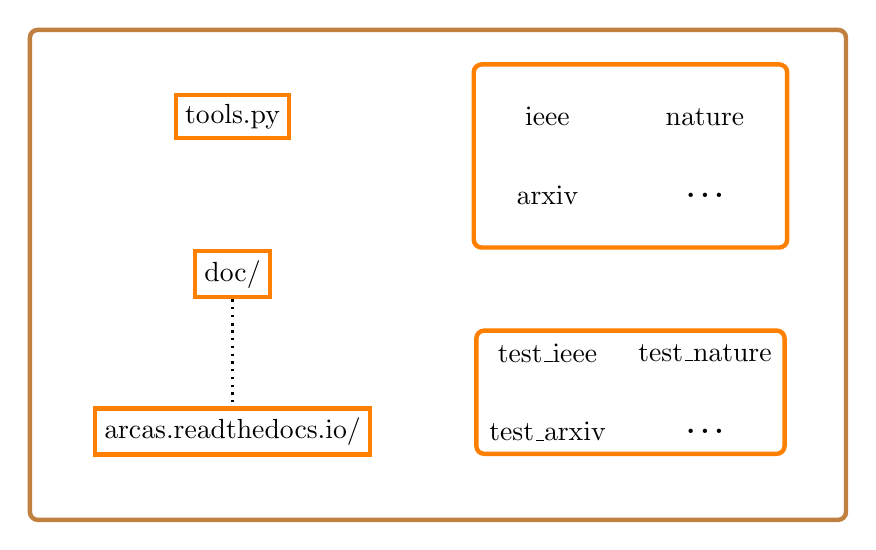
\begin{tikzpicture}

\tikzstyle{state}=[minimum width=0.4cm, font=\boldmath];
    

    \node[ultra thick, draw=orange] (0) at (0, 0) [state] {tools.py};
    \node[ultra thick, draw=orange] (1) at (0, -2) [state] {doc/};

    \node[ultra thick, draw=orange] (2) at (0, -4) [state] {arcas.readthedocs.io/};

    \node[ultra thick] (3) at (4, 0) [state] {ieee};
    \node[ultra thick] (4) at (6, 0) [state] {nature};
    \node[ultra thick] (5) at (4, -1) [state] {arxiv};
    \node[ultra thick] (6) at (6, -1) [state] {$\dots$};  

    \node [background, inner sep=4mm, fit=(3) (4) (5) (6)] {};

    \node[ultra thick] (7) at (4, -3) [state] {test{\_}ieee};
    \node[ultra thick] (8) at (6, -3) [state] {test{\_}nature};
    \node[ultra thick] (9) at (4, -4) [state] {test{\_}arxiv};
    \node[ultra thick] (10) at (6, -4) [state] {$\dots$};  

    \node [background, fit=(7) (8) (9) (10)] {};

    \draw (1) edge[out=-90, in=90, -, thick, dotted] node [above] {} (2);

    \node [background, brown, inner sep=8mm, fit= (0) (1) (2) (3) (4) (5) (6) (7) (8) (9) (10)] {};

\end{tikzpicture}
\end{document}
\end{figure}
\end{center}
\end{frame}

\begin{frame}[fragile]
    \begin{minted}
    [
    framesep=4mm,
    baselinestretch=1.2,
    bgcolor=DarkGray,
    fontsize=\scriptsize,
    ]
    {python}
$ arcas_scrape --version
Arcas 0.0.3
    \end{minted}
\vspace{0.5cm}
    \begin{minted}
    [
    framesep=4mm,
    baselinestretch=1.2,
    bgcolor=DarkGray,
    fontsize=\scriptsize,
    ]
    {python}
$ arcas_scrape -p arxiv -t "Sustainable Software" -r 1
http://export.arxiv.org/api/query?search_query=ti:Sustainable 
Software&max_results=1&start=1
    \end{minted}
\end{frame}

\begin{frame}
    \begin{center}
        \small{@NikoletaGlyn}\\
        \small{https://github.com/ArcasProject/Arcas} \\
        \small{https://nikoleta-v3.github.io}
    \end{center}
\end{frame}

\end{document}